\documentclass{article}
\usepackage[utf8]{inputenc}
\usepackage{lmodern}
\usepackage{amsmath}
\usepackage{hyperref}
\usepackage{bm, graphicx}
\usepackage[a4paper, margin=1in]{geometry}

\begin{document}
	
\title{Analytical Questions}
\author{Afarin Fatemeh Rezaei}
\date{\today}
\maketitle

	
\begin{enumerate}
	\item \textbf{Relationship Between Density of States (DOS) and Band Structure}
	\begin{enumerate}
		\item
		Peaks in the density of states (DOS) arise at energies where there are many bands very close in energy, often because of band degeneracy or flatness. These points in the Brillouin zone correspond to places where the electronic dispersion is minimal, and the group velocity vanishes. Such features give rise to what are known as \emph{Van Hove singularities}~\cite{vanhove} in the DOS: sharp increases or divergences in the density of states due to critical points (maxima, minima, saddle points) in the band structure.
		\item
		Flat bands in the band structure (i.e., bands that do not disperse much with wave vector \( k \)) result in a large accumulation of electronic states at a given energy, since many \( k \)-points correspond to nearly the same energy. This leads to pronounced peaks in the DOS at those energies, a direct manifestation of Van Hove singularities~\cite{ashcroft_mermin,martin}.
	\end{enumerate}
	
	\item \textbf{Conductivity Analysis}
	\begin{enumerate}
		\item
		The energy gap between the valence band maximum and the conduction band minimum, as measured from the band structure plot, defines the fundamental band gap of the material. For silicon, this indirect band gap is experimentally about 1.1\,eV at room temperature; however, typical DFT calculations often underestimate it, yielding a gap of approximately 0.6\,eV~\cite{kittel}. The band gap present in my calculation (see file BANDSTRUCTURE.py output) is at 0.6480\,eV with valence band maximum (VBM) at -0.0001\,eV and
		conduction band minimum (CBM) at 0.6479\,eV
		\item
		Because this band gap is finite and the Fermi energy lies within the gap, silicon is a \emph{semiconductor}. If the valence and conduction bands overlapped (zero or negative gap), the material would be metallic. A much larger gap (e.g., several eV) would indicate an insulating material~\cite{ashcroft_mermin}.
	\end{enumerate}
	
	\item \textbf{Interpretation of DOS, PDOS, and Band Structure}
	\begin{enumerate}
		\item
		The DOS plot provides information about the distribution of electronic states across different energies. Peaks highlight the energies where many states are available (e.g., due to flat or degenerate bands), while valleys represent energy regions with few available states.
		\item
		The projected density of states (PDOS) separates the contributions from different atomic orbitals or atoms to the total DOS. For example, analyzing the PDOS of silicon can reveal how the \( s \) and \( p \) orbitals contribute to different portions of the electronic spectrum, and hence to chemical bonding and optical properties.
		\item
		The band structure plot shows how electron energies vary as a function of momentum in the crystal (along specific symmetry directions). Highly dispersive bands (steep slopes) indicate delocalized electrons with high mobility, characteristic of good conductors or semiconductors. Flat bands indicate localized electronic states and higher effective mass. The presence or absence of a band gap allows classification of the material as a metal, semiconductor, or insulator.~\cite{ashcroft_mermin,kittel}
	\end{enumerate}
\end{enumerate}
	
	\begin{thebibliography}{99}
		\bibitem{vanhove}
		L. Van Hove, ``The Occurrence of Singularities in the Elastic Frequency Distribution of a Crystal,'' \textit{Phys. Rev.} \textbf{89}, 1189 (1953).
		\bibitem{ashcroft_mermin}
		N. W. Ashcroft, N. D. Mermin, \textit{Solid State Physics}, Brooks Cole, 1976.
		\bibitem{kittel}
		C. Kittel, \textit{Introduction to Solid State Physics}, 8th Edition, Wiley, 2004.
		\bibitem{martin}
		R. M. Martin, \textit{Electronic Structure: Basic Theory and Practical Methods}, 2nd Ed., Cambridge University Press, 2020.
	\end{thebibliography}
	

	
	\begin{figure}[h]
		\centering
		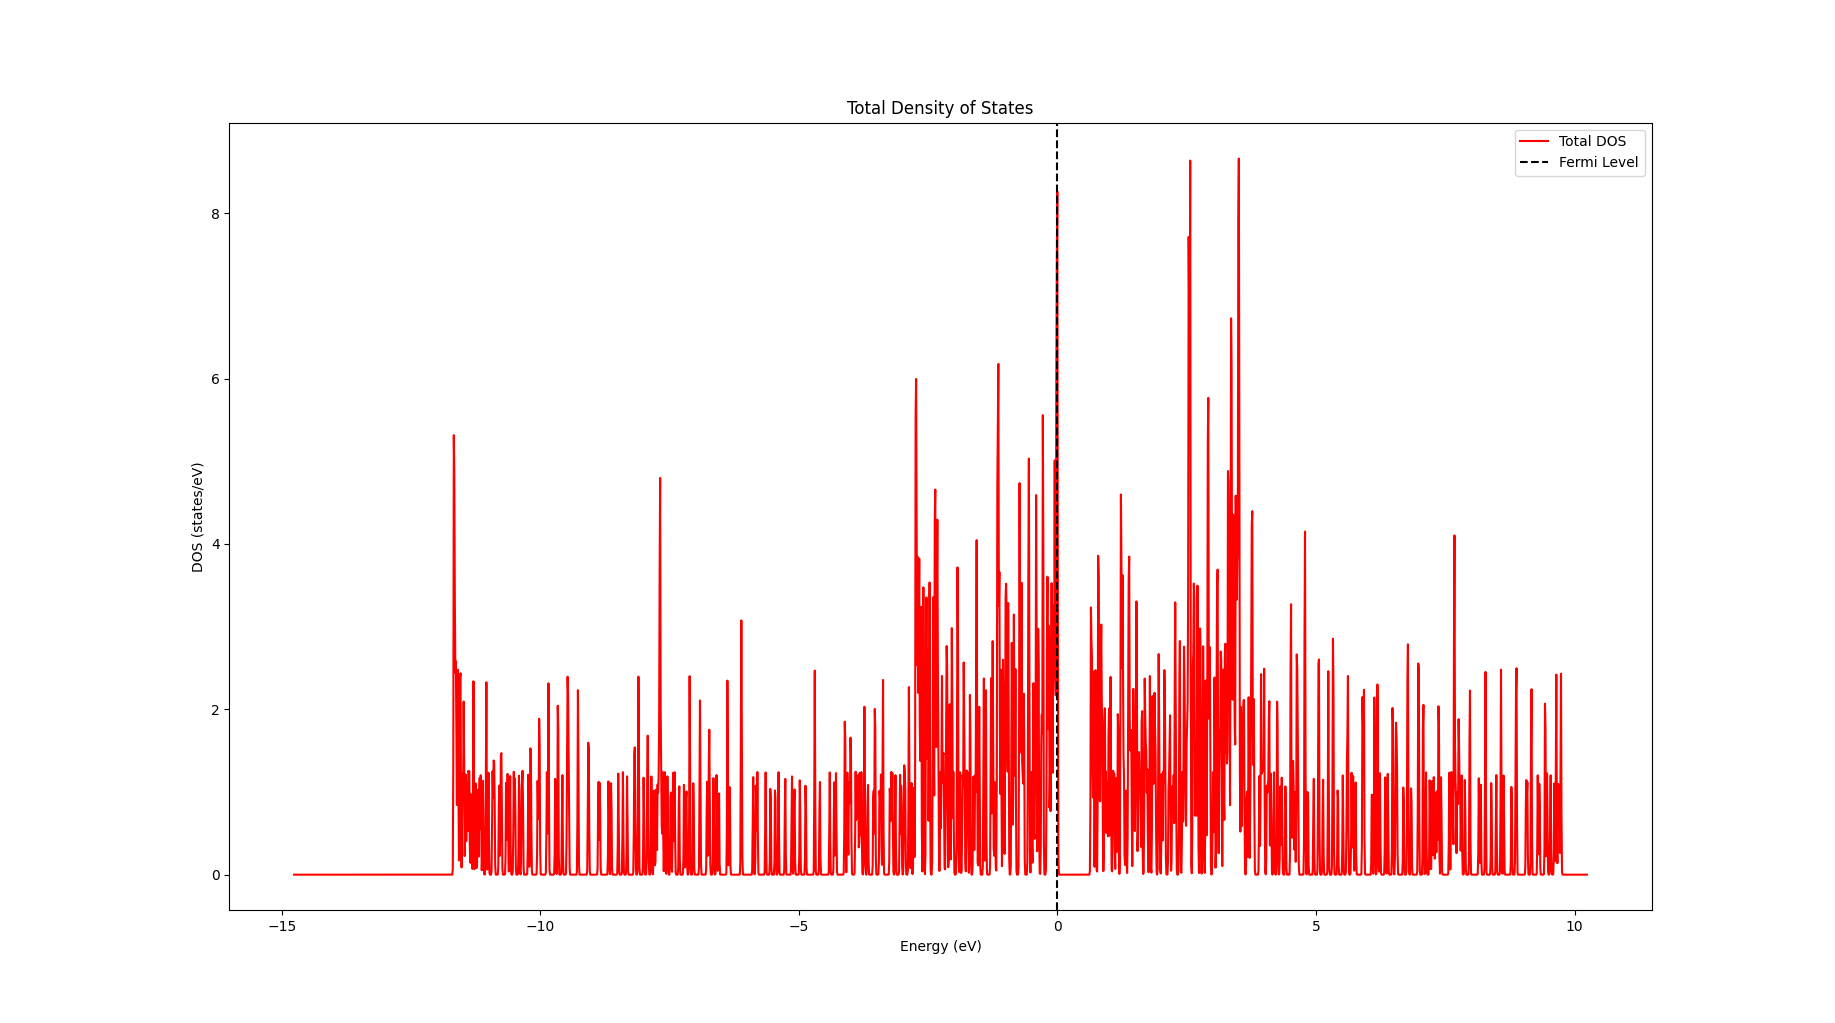
\includegraphics[width=1\linewidth]{DOS.png}
		\caption{Total DOS showing van Hove singularities}
		\label{fig:dos}
	\end{figure}
	

	
	\begin{figure}[h]
		\centering
		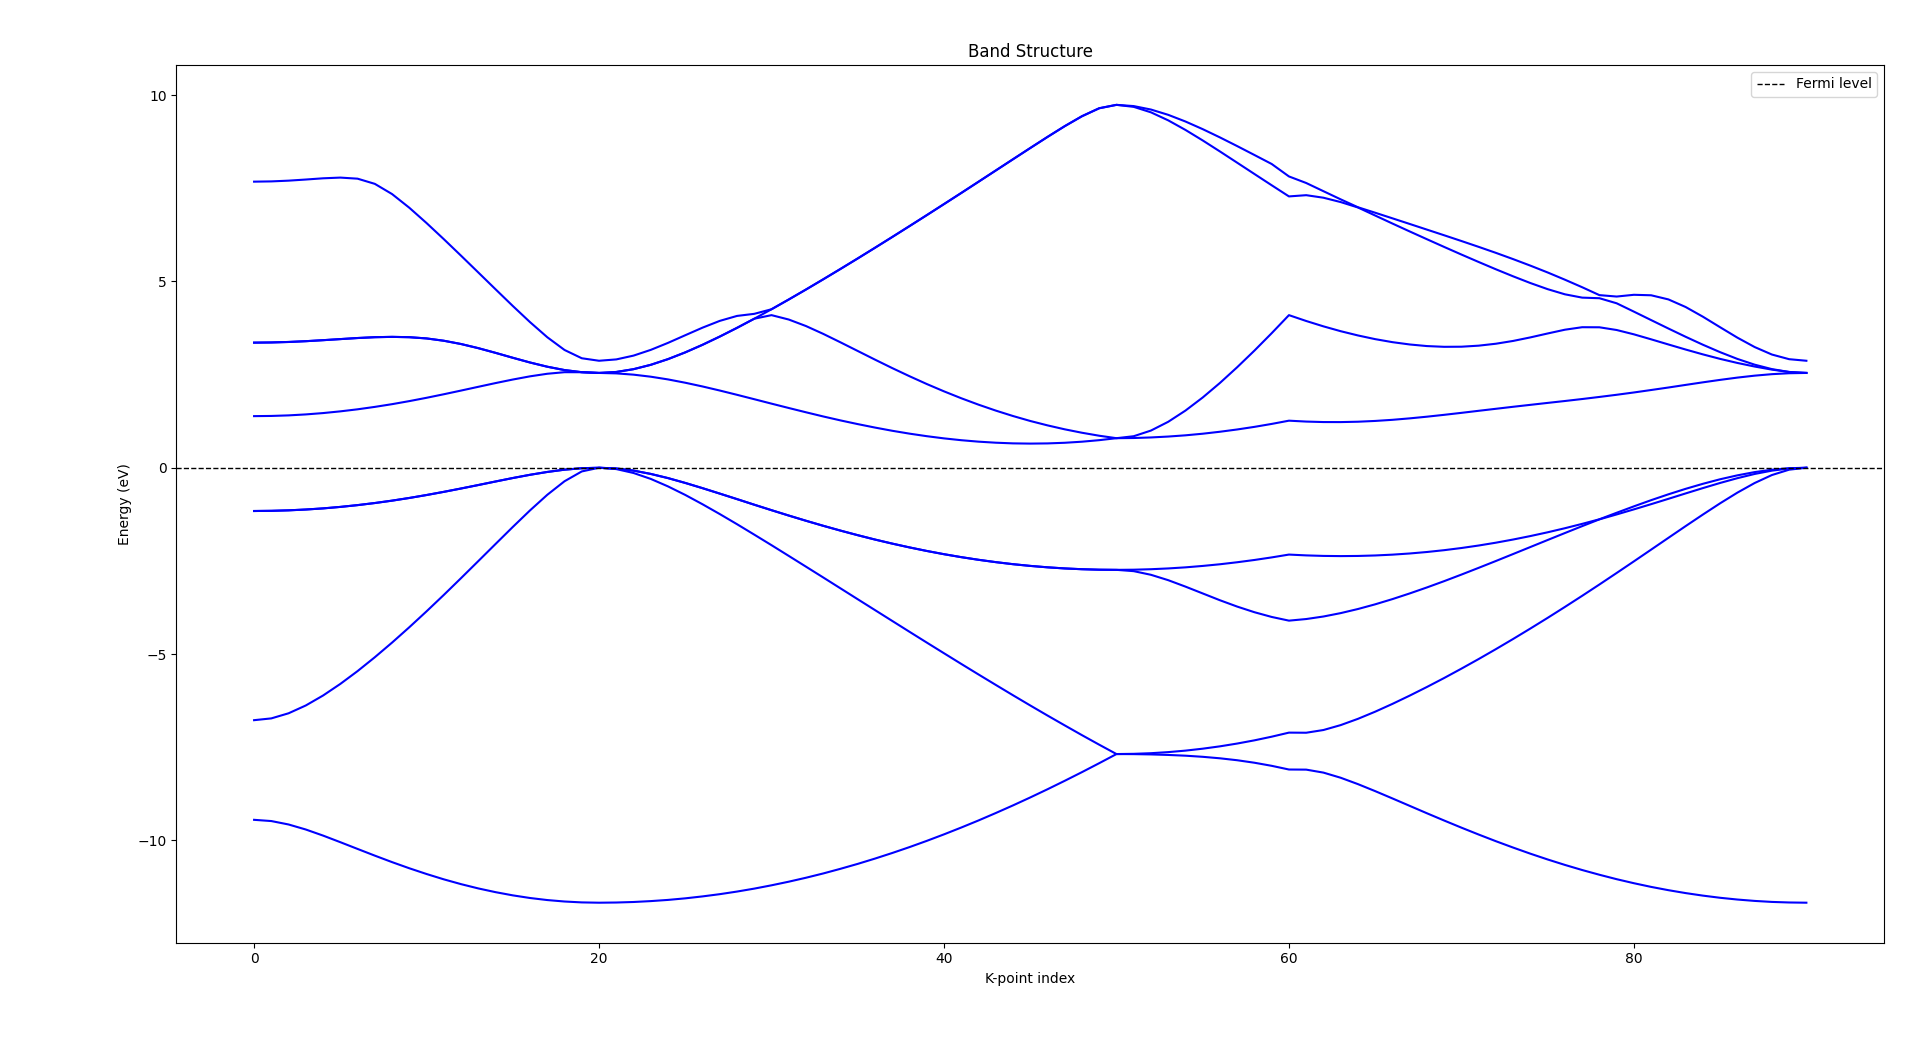
\includegraphics[width=0.9\linewidth]{BandStructure.png}
		\caption{Band structure showing bandgap}
		\label{fig:band}
	\end{figure}
	


	\begin{figure}[h]
		\centering
		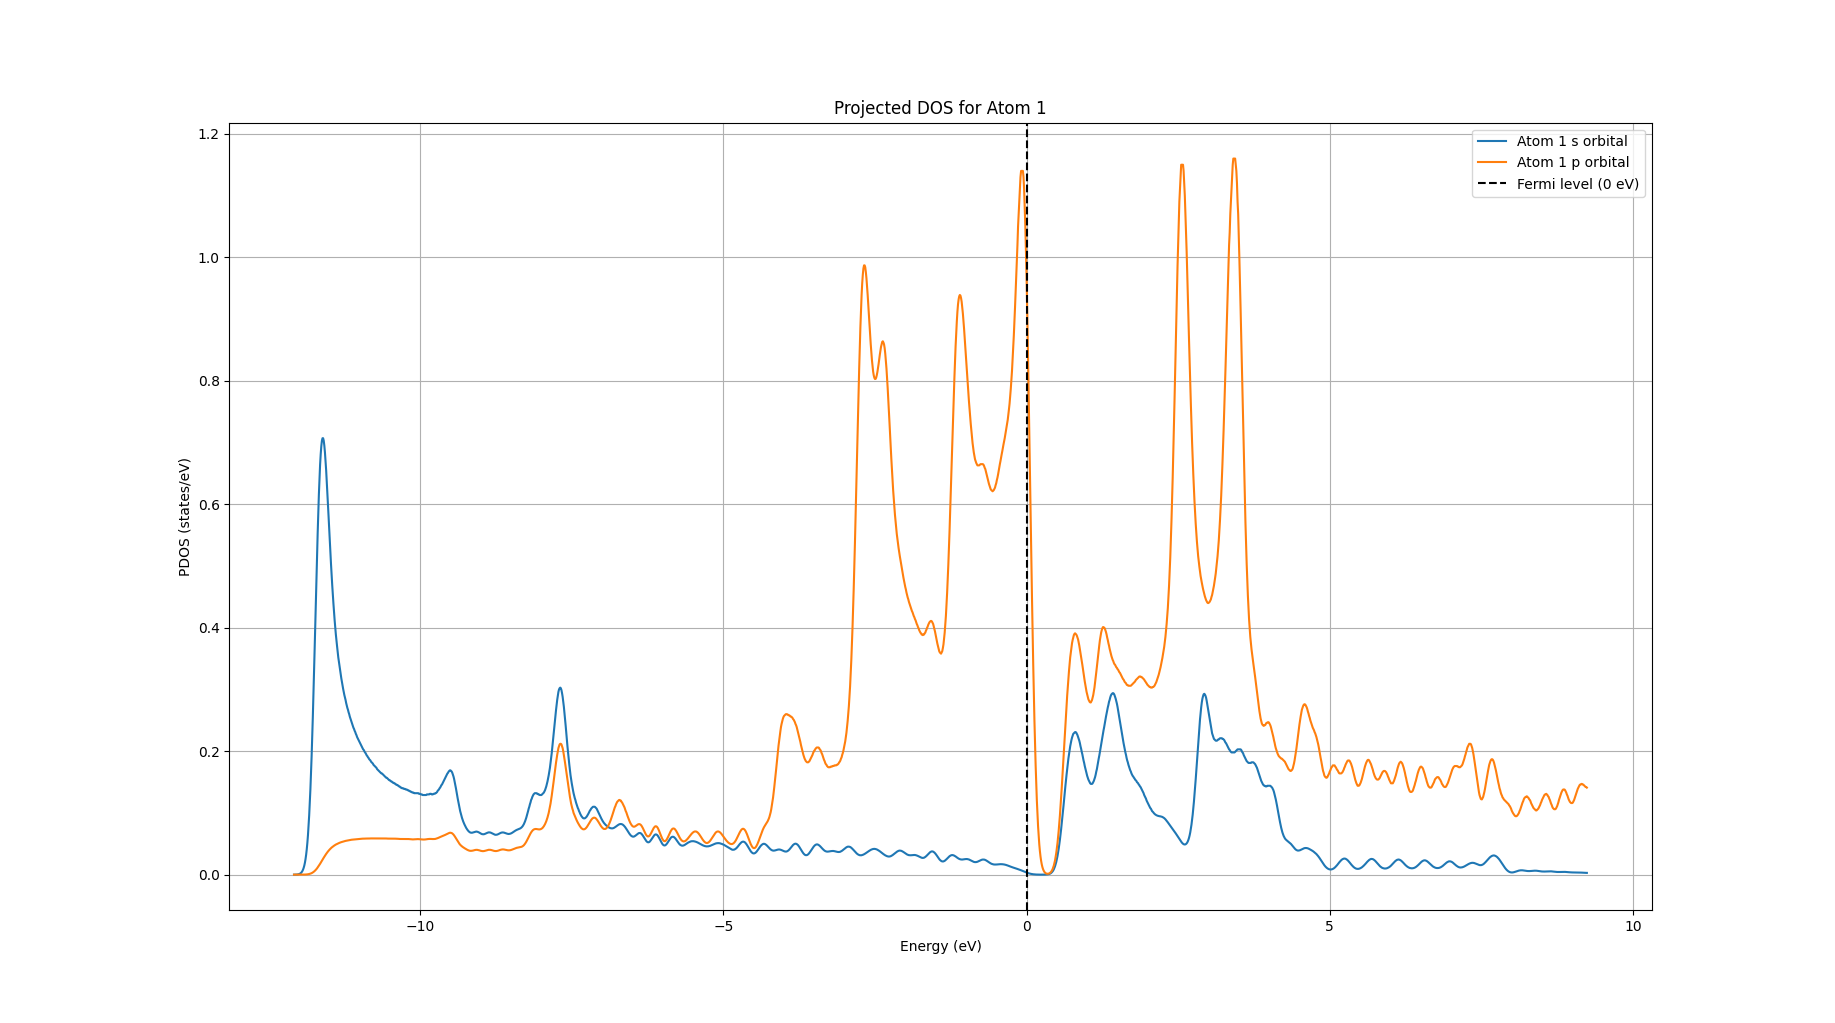
\includegraphics[width=1\linewidth]{PDOS(atm1).png}
		\caption{Atom 1 PDOS}
		\label{fig:pdos1}
	\end{figure}
	\hfill
	\begin{figure}[h]
		\centering
		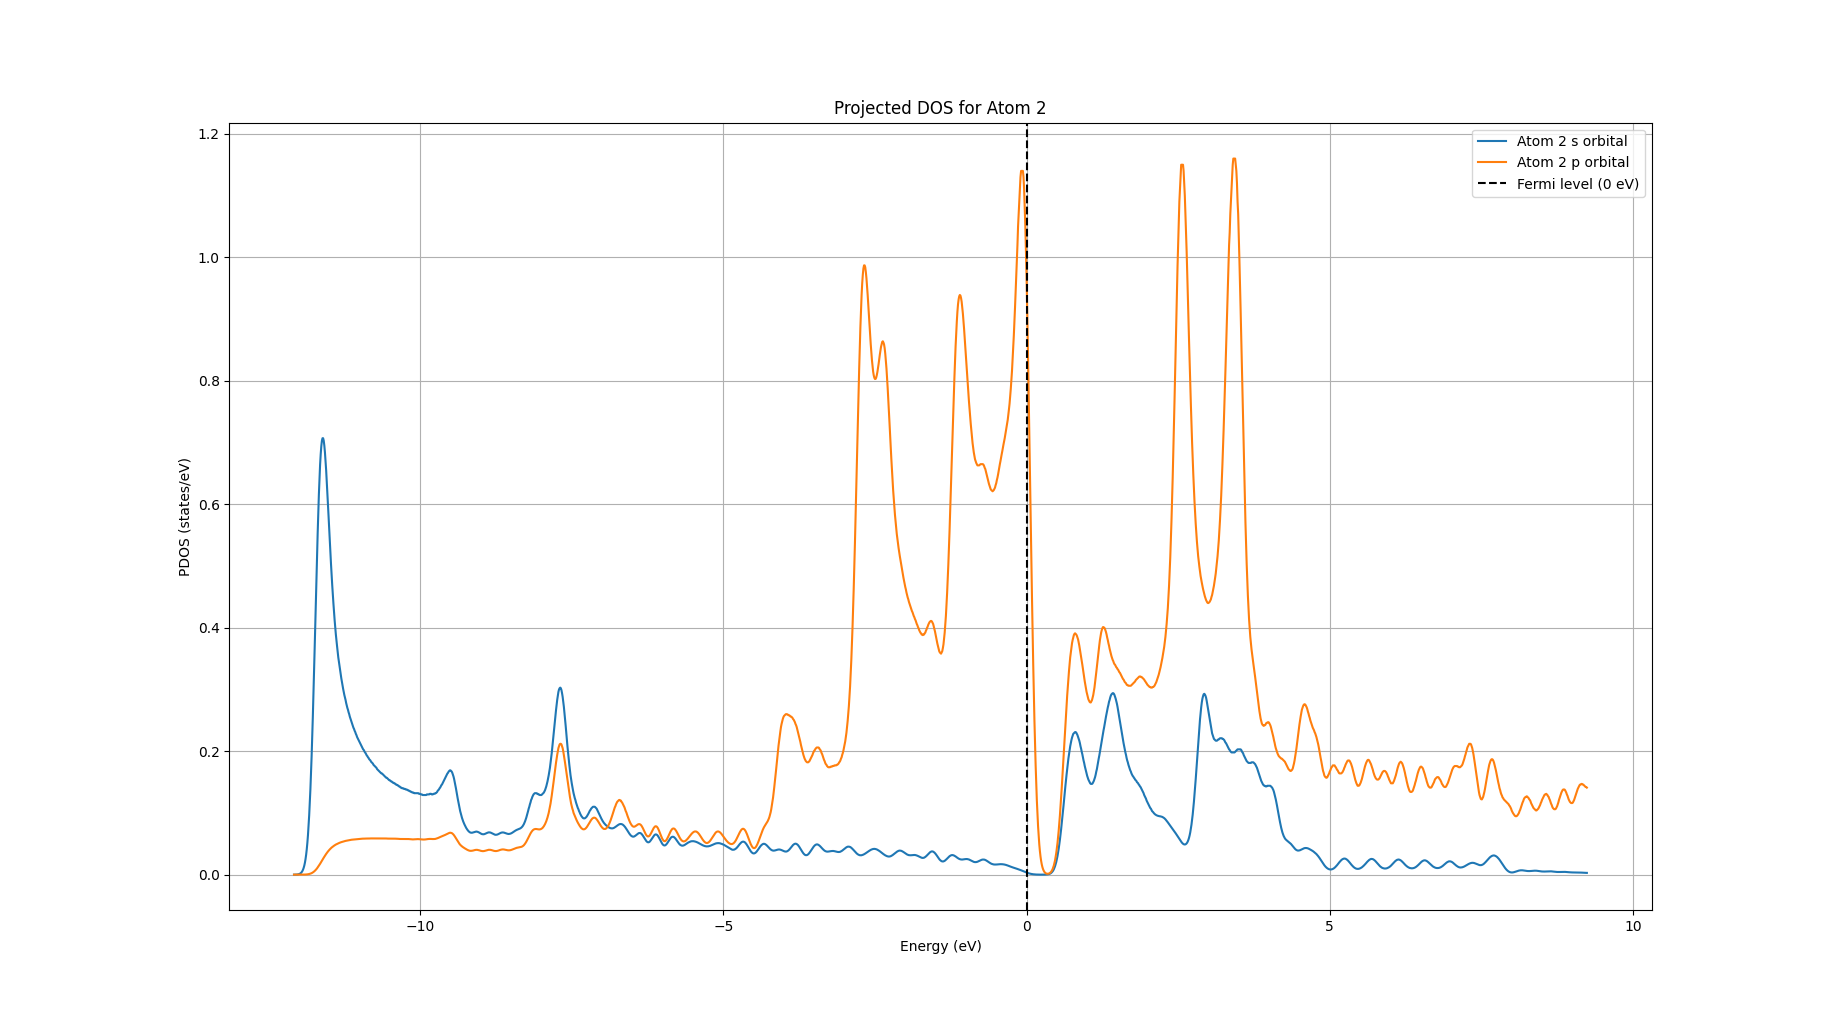
\includegraphics[width=1\linewidth]{PDOS(atm2).png}
		\caption{Atom 2 PDOS}
		\label{fig:pdos2}
	\end{figure}
	
	\begin{figure}[h]
	\centering
	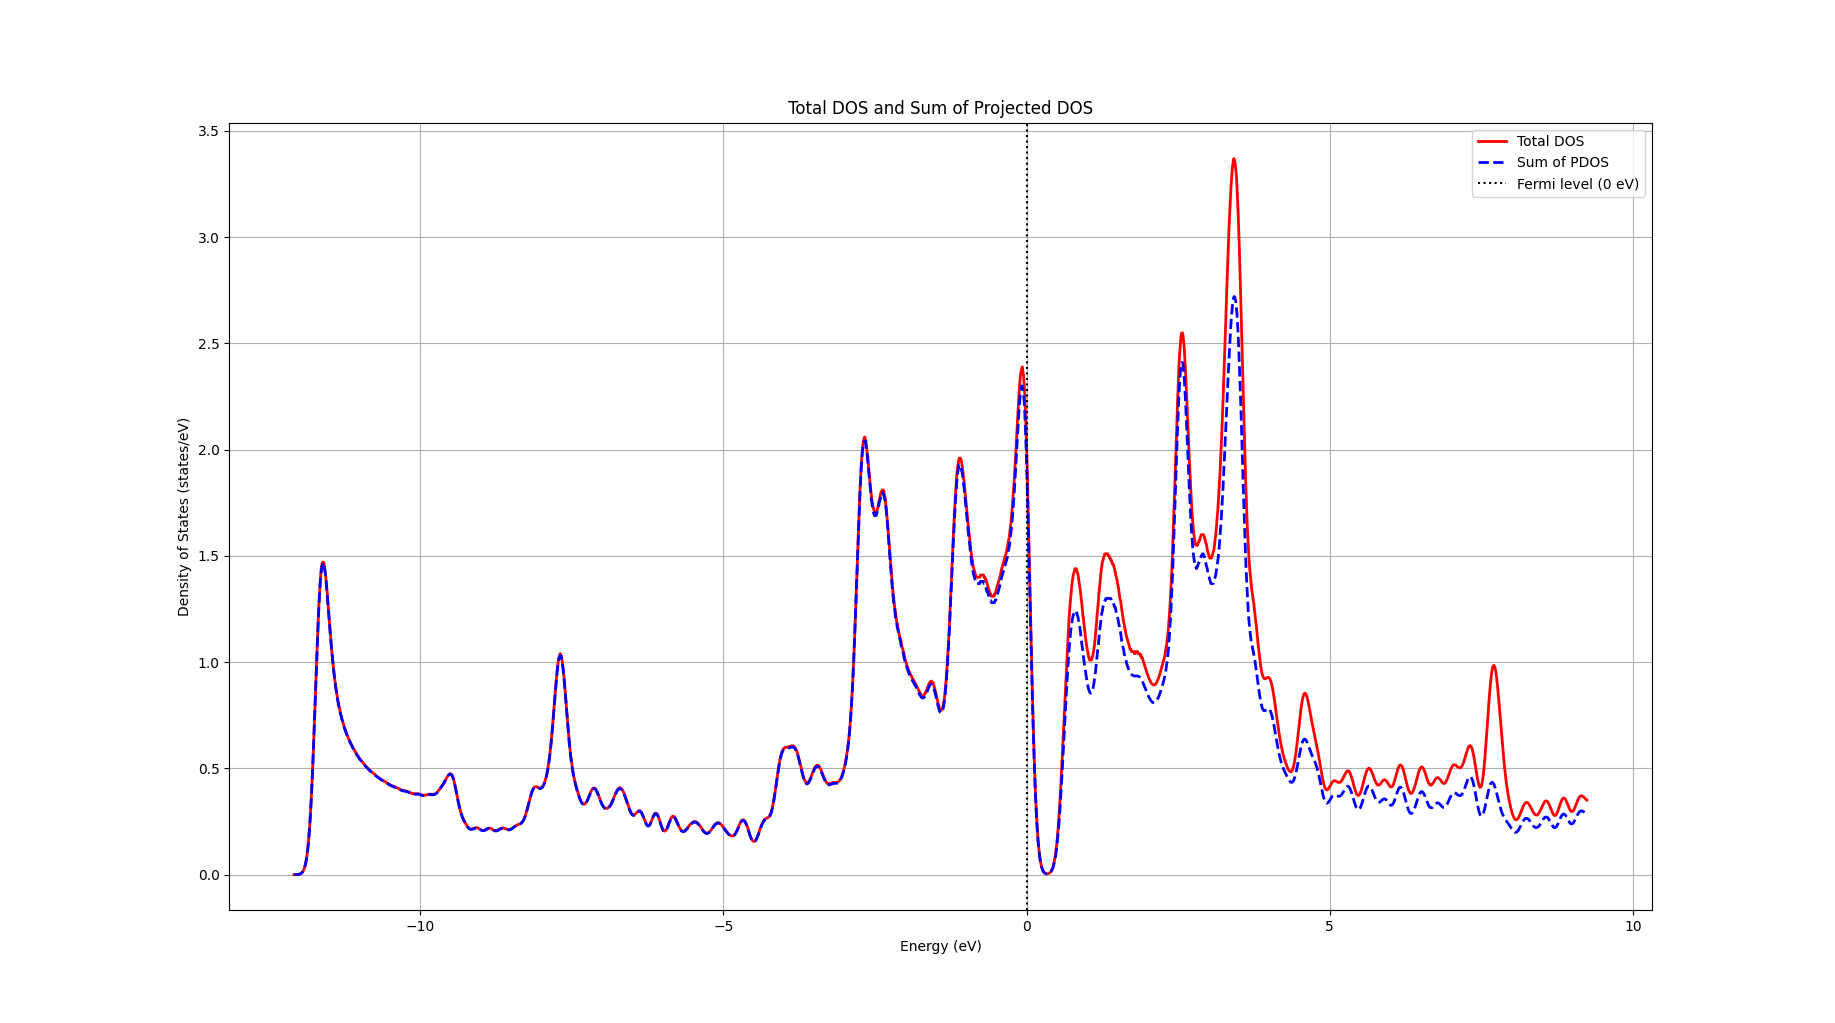
\includegraphics[width=1\linewidth]{DOSvsPDOS.png}
	\caption{The comparison between DOS and PDOS}
	\label{fig:pdos3}
\end{figure}

\end{document}